\section{Our Thoughts Determine Our Lives}

Cologero had mentioned this book\footnote{\url{https://www.amazon.com/Our-Thoughts-Determine-Lives-Teachings/dp/1887904190}}, coincidentally, at the same time that I had stumbled across it myself, so I finally made the purchase, and finished reading it. I found it most helpful; Elder Thaddeus\footnote{\url{https://orthodoxwiki.org/Thaddeus_\%28Strabulovich\%29_of_Vitovnica}} is simultaneously very strict (insofar as he sets out an arduous teaching\footnote{\url{http://www.orthodoxengland.org.uk/pdf/thaddeus.pdf}}) and yet very compassionate, encouraging, and “human”: at one point, the man even had a cigarette problem, which he overcame, while in Kosovo at the Pech monastery. Elder Thaddeus was not a legalistic or judgmental man – what he was, most definitely, was a saint.

\begin{wrapfigure}{rt}{.3\textwidth}
 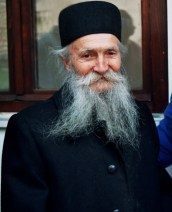
\includegraphics[scale=.6]{a20130412OurThoughtsDetermineOurLives-img001.jpg}
\end{wrapfigure}

Apparently, Elder Thaddeus had several experiences with angels, one while wide awake in prison, in which a very tall man wearing an old military uniform with a strange gold cross came to him to assure him that the Nazis would not be executing him, because God had many in Serbia that needed comfort. He also experienced the prayer “in” or “by” the heart through the Jesus prayer, and attained all three levels of Orthodox mystical experience by the time of his death. At his funeral, the birds, of whom he had often spoken with love and admiration, came in great numbers.

Here are some important points of doctrine gleaned from his essays, topical sermons, and quotes (ie., these are points that are repeated in various contexts and ways).

\begin{enumerate}

\item Man is a spiritual being who is dominated by psychic delusion and bodily passions, which convince us that “we” need something that is superfluous.

\item This domination always occurs through the power of aerial spirits, which are fallen angels, who have access to man's psychic constitution and long experience in manipulating man.

\item These spirits have varying degrees of wickedness, even among their own hierarchy.

\item They do this because they are lonely, fearful of the coming judgement, envious of man's special and privileged status, and because they also “feed” off the psychic energy derived from man's falling into sin. Each angel or spirit has their own “specialty”.

\item Man has the power to resist this, primarily because these spirits cannot access or even see man's inner heart, and because God Himself intervenes very frequently to lead souls back to Him.

\item God knew that the original state of man would “fall”, and that we would not be able to maintain our perfection; He therefore wisely and compassionately determined to use His own nature, and ours, in a synergistic way to overcome the fall, to lead back certain souls who remembered Him despite their sins, through their educative process back to a pristine condition.

\item This synergism is most boldly seen in the figure of Christ, who is the archetype or pattern for what will come after.

\item Mary the Theotokos is the pattern for what our love for God should be like. (I will speculate that this is primarily due to the lack of perfection in Christ, and the “feminine” nature of our soul in relation to its higher parts/God). Christ is the eventual pattern for our love, but Mary is chief among the saints.

\item Communion with angels and saints is necessary in order to achieve communion with God.

\item No evil spirit can touch someone who hasn't first harmed themselves. “We are the sole architects of our future”.

\item Everyone without exception desires absolute life and love: humans are variously warped in their search for this.

\item Vigilance, eternal vigilance, is necessary to achieve a state of grace, and even to keep it. You must examine every thought that enters your inner heart.

\item Only through the descent of the higher part of the soul, the Nous, into the heart, can a state of illumination be achieved. This state can be prepared for, and God will grant it, but only when the time is right (ie., when someone has a chance of keeping it, and/or not abusing it for evil ends).

\item Obedience and vigilance are greater virtues than fasting and even prayer, unless the prayer comes from the heart (or, greater, is “of” the heart).

\item God will listen to any prayer from the heart, even if someone is very far from Him.

\item The evil spirits try very hard to separate children from parents, because this fracture of Tradition and custom accomplishes the loss of moral knowledge, spiritual truth, and the blessing that naturally adheres to filial obedience.

\item Men are “thought generators and receptors” : our thoughts have power and being – they influence us, and ours influence others:

\begin{quotex}
Your thoughts are burdened because you are influenced by the thoughts of your fellow men. Pray to the Lord that He might take this burden from you. These are the thoughts of others which differ from yours. They have their plan, and their plan is to attack you with their thoughts. Instead of letting go, you have allowed yourself to become part of their plan, so of course you suffer.
Had you ignored the attack, you would have kept your peace.
They could have thought or said anything at all about you, yet you would have remained calm and at peace.
Soon all their anger would have died down, like a deflated balloon, because of the pure and peaceful thoughts that would have come from you.
If you are like that, calm and full of love, if all you think are good and kind thoughts, they will stop warring against you in their thoughts and will not threaten you anymore.
But if you demand an eye for an eye, that is war.
Where there is war there can be no peace.
How can there be peace on a battlefield, when everyone is looking over their shoulders and anticipating a surprise attack from the enemy?

\end{quotex}

\item Love comes from God, passion comes from evil spirits; men are constantly confusing and mixing the two. When we do this, evil predominates.

\end{enumerate}

\textit{Addendum:} So as not to cause those of the warrior caste to stumble, I point out that Orthodoxy does not have, as saints, exclusively Brahmins. There are warrior saints as well. There is an interesting tale mentioned by Elder Thaddeus in his book: the Turks once summoned at a parley the Serbs, and reproached them for not submitting to their rule, as their Christian faith should dictate (does this sound like secular humanists lecturing Christians on the faith?). They wanted to know by whose leave they fought, as Christians. The Serbs explained that the Lord commanded them to turn the other cheek as individuals, but that they were given a mission to guard those under their care, their families and small ones, so that by fighting in battle, they were doing double service to Christ in protecting and loving those under their responsibility.


\flrightit{Posted on 2013-04-12 by Logres }

\begin{center}* * *\end{center}

\begin{footnotesize}\begin{sffamily}

\texttt{CaseyAnn on 2013-04-13 at 14:40 said: }

Please, will you explain what you mean by ``the lack of perfection in Christ''? I'm not sure to what you are alluding, but this specifically\footnote{\url{http://newtheologicalmovement.blogspot.com/2013/01/christ-did-not-grow-in-grace-or-in.html}} comes to mind.


\hfill

\texttt{Logres on 2013-04-13 at 22:05 said: }

The Orthodox (I think?) would say that since Christ is Deity, we sometimes feel more alienated from Him than we should, due to His exalted condition and our sinful one; therefore, prayers to the saints and angels (particularly Mary) can be made as a way of approaching to Christ. Perfect love casts out fear, so someone who serves God as a son has Christ as an older brother, and is at the top of the three stages of progress. However, there are two others: 2) those who serve for the reward 3) those who serve as slaves, out of fear. The spirituality will look differently for each; on the one hand, all who believe are perfected in potential (and perhaps actually, if we take an eternal view). On the other, St Paul speaks of “Christ being formed in us”, and not wanting that to be marred or taken away prior to its (presumed?) perfection.

So, yes, if Christ grew in holiness, we would expect to have to do the same, to achieve greater perfections, although this is not precisely what I meant. Sinners advance analogously in terms of hierarchy, but not ontology, since He was born flawless to begin with. 

But the over-arching analogy is valid, to the degree the difference is seen.


\hfill

\texttt{CaseyAnn on 2013-04-14 at 02:28 said: }

Ah, I see I completely misread you. I read that as “Jesus Himself lacks perfection,” as opposed to “we lack perfection in Him.” Thank you for the clarification. 

And yes, I've heard reliance on Mary's intercession explained, based on Saint Louis de Montfort's True Devotion to Mary, as that some souls experience shame when turning to Christ for mediation to the Father and, therefore, may seek Mary to mediate between them and her Son. I can understand the sense of being unworthy to approach His holy dignity, but the explanation certainly felt wrong, in terms of lacking.

Does that mean, then, that it is actually spiritually superior to “go straight to Jesus!” (ha), as opposed to through another mediator? Or does that depend on the spirituality (hierarchically) of the individual? It's a curious speculation, as so many followers of the perverted forms of Christianity never, at any point, seek intercession from the angels and saints above.


\hfill

\texttt{Logres on 2013-04-14 at 06:15 said: }

Casey-Ann, I would incline to the latter; although certainly the abuses of appealing to saints/angels have been highlighted during the Reformation and by its followers, it never seems to have occurred to them at any point to wonder if the “Jesus alone” could have its own abuses, and if they were (perhaps) on balance worse. 1) Jesus is reduced to microscopic size (you see this in the casual attitude and secularism 2) He now has no family 3) no hierarchy exists. For many, you have to conclude that this is the actual appeal! They also lie and distort the teachings of liturgical Churches: there is a critical attitude with no charity or attempt to see the deeper meaning. This is an even worse sin. 

If we follow Protestant logic, it's superior to go straight to God; but then again, it's superior to that to believe in no God at all, go straight to yourself. Of course, all this is is a perversion and misappropriation of Tradition's teachings, or “cheap grace”. In reality, it all depends on the inner state of the individual (which is not “relative” in the modern sense) as to what practices are appropriate to the “hidden soul”. 

Thank you for the thoughtful comments.


\hfill

\texttt{Caleb Cooper on 2013-04-14 at 17:41 said: }

The protestant desire to “go straight to God” makes me think of someone who knows that light is good and necessary for life, so they want to look straight into the the Sun and fly like Icarus directly to it. 

St. Paul experienced what happens when one gets to close to the light of the Son; the result would be blindness, sunburn, and eventually incineration far before one even got close to the goal if one persisted in such a foolhardy course. “No one can see the face of God and live.” (though as Logres points out, the most common result for the protestant is that they instead substitute a reduced concept of God) 

The Christian/Traditionalist ambition is to forge a spirit strong enough to survive seeing God face to face in love. It's a task more difficult than the analogous one of being able to build a spaceship capable of safely flying/burrowing safely all the way into the center of the Sun (which is an impossible feat for physical engineering).

(My soul apparently can't even reach the heart of God, let alone His beatific face. The height to which the soul can ascend is proportional to its density. When I ascend I can't get past what would correspond to the third chakra in God, because my soul's density is to heavy for it to go further. Such is my soul's current state; there is too much `ossified' energy in my third chakra that interferes with energy rising up to and fully developing the heart chakra (a very common distortion of the soul in the modern world)) 

I also once had a very interesting experience when my spirit `woke up.' It was very bizarre, seeing a me acting independently of it's own volition. It put me in a safe sphere, and then proceeded to do something incredbily stupid; it tried to get forcibly back to Heaven by flying into the Light. Huge amounts of darkness began peeling off it as it ground against some invisible barrier. My spirit was quite persistent, but eventually it reached it's limit and fell back down into the dark depths of the waters, which was an extremely unpleasant experience to come out of. It was kinda funny afterwords though; “Great, my higher soul woke up, but it turns out that while he may be earnest he's also a total moron.”

“Or does that depend on the spirituality (hierarchically) of the individual?”

As always, know thyself. Even for an individual it can change from occasion to occasion what is the appropriate way to access heaven. The key in all things spiritual is establishing resonance in the heart. 

This is another reason besides shame why the saints and angels can be so useful: the distance between us and God/Christ is so great that we can have a hard time coming into resonance with them, while we may be more able to identify with certain saints or angelic beings. 

While God's power is greater, if we fail to tune in it's less likely that this power will be activated, so it's better to ask for intercession from a being whom we can achieve resonance with. And in coming closer to them we will eventually become closer to God, our soul slowly becoming stronger so we can some day stand before God under our strength. To throw out the saints and angels is to dispense with a valuable ladder that helps support us in our climb toward heaven.


\hfill

\texttt{CaseyAnn on 2013-04-16 at 18:12 said: }

“The height to which the soul can ascend is proportional to its density. . . there is too much `ossified' energy in my third chakra that interferes with energy rising up to and fully developing the heart chakra (a very common distortion of the soul in the modern world))”

Your last comment particularly resonated with my worry that the godlessness to which we are exposed in the modern world “distorts” our souls in an irreversible manner while on Earth. But all things are possible, so this cannot be, right?

I appreciate your lengthy reply.


\hfill

\texttt{CaseyAnn on 2013-04-16 at 18:23 said: }

Logres, thank you. “Cheap grace” sadly explains it well. I read a strange comment by a Protestant once about Christians not having differing “net grace”; basically, his idea was that we are all equal in the amount of grace because it would be absurd to imagine grace as being granted in amounts, or something to that effect. This is to what he tried to reduce spirituality. And the conversation was about this very topic.

I think it exemplifies the 3 points you made, in that very order: “1) Jesus is reduced to microscopic size (you see this in the casual attitude and secularism 2) He now has no family 3) no hierarchy exists.”


\hfill

\texttt{zetjintsu on 2013-04-17 at 12:46 said: }

@CaseyAnn: Indeed, have faith; “and Jesus looked at them and said, “With man this is impossible, but with God all things are possible.” (Matthew 19:26)

It is a common feeling that we have become irredeemably damaged goods, but behind this feeling is a rather egoistical belief that shows a lack of faith that God is the Almighty, the belief that our capacity for sin is more powerful than God's capacity for a love which conquerors and transforms all. 

“Love never fails.” God's love never fails. “Beloved, do not forget this one thing… God is not slack fulfilling His promises as some count slackness, but is long suffering toward us; He is not willing that any should perish, but that all should be saved.” (2 Peter 3:8) Can God fail to fulfill His will? This question and scripture can be a powerful meditation when you find your faith faltering and worry that your soul could be “distorted” in a manner irreversible by God's grace. 

Pray to the saints that you may have faith like unto theirs. Remember that the church father's teach that faith is the foundation on which all else is built. Tradition is cooperation between heaven and earth, and faith is what opens our heart to divine grace and discernment of its will.


\end{sffamily}\end{footnotesize}
